\documentclass[a4paper]{article}
\usepackage[spanish]{babel}
\usepackage[utf8]{inputenc}
\usepackage{charter}   % tipografia
\usepackage{graphicx}
\usepackage{wrapfig}
\usepackage[dvipsnames]{xcolor}
\usepackage{textcomp}

\usepackage{color} % para snipets de codigo coloreados
\usepackage{fancybox}  % para el sbox de los snipets de codigo

\definecolor{litegrey}{gray}{0.94}

% \newenvironment{sidebar}{%
% 	\begin{Sbox}\begin{minipage}{.85\textwidth}}%
% 	{\end{minipage}\end{Sbox}%
% 		\begin{center}\setlength{\fboxsep}{6pt}%
% 		\shadowbox{\TheSbox}\end{center}}
% \newenvironment{warning}{%
% 	\begin{Sbox}\begin{minipage}{.85\textwidth}\sffamily\lite\small\RaggedRight}%
% 	{\end{minipage}\end{Sbox}%
% 		\begin{center}\setlength{\fboxsep}{6pt}%
% 		\colorbox{litegrey}{\TheSbox}\end{center}}

\newenvironment{codesnippet}{%
	\begin{Sbox}\begin{minipage}{\textwidth}\sffamily\small}%
	{\end{minipage}\end{Sbox}%
		\begin{center}%
		\colorbox{litegrey}{\TheSbox}\end{center}}



\usepackage{fancyhdr}
\pagestyle{fancy}

%\renewcommand{\chaptermark}[1]{\markboth{#1}{}}
\renewcommand{\sectionmark}[1]{\markright{\thesection\ - #1}}

\fancyhf{}

%\fancyhead[LO]{Sección \rightmark} % \thesection\ 
\fancyfoot[LO]{\small{Juan Lanuza, Agustin Penas, Fernando Frassia}}
\fancyfoot[RO]{\thepage}
\renewcommand{\headrulewidth}{0.5pt}
\renewcommand{\footrulewidth}{0.5pt}
\setlength{\hoffset}{-0.8in}
\setlength{\textwidth}{16cm}
%\setlength{\hoffset}{-1.1cm}
%\setlength{\textwidth}{16cm}
\setlength{\headsep}{0.5cm}
\setlength{\textheight}{25cm}
\setlength{\voffset}{-0.7in}
\setlength{\headwidth}{\textwidth}
\setlength{\headheight}{13.1pt}

\renewcommand{\baselinestretch}{1.1}  % line spacing


\usepackage{underscore}
\usepackage{caratula}
\usepackage{url}
\usepackage{float}


\usepackage{listings}


\renewcommand{\lstlistingname}{C\'odigo}
\lstloadlanguages{[ANSI]C} 
\lstset{language=[ANSI]C,
        frame=single,
        breaklines=true, 			% Saltar de linea si supero el maximo
        basicstyle=\small\ttfamily,
        keywordstyle=[1]\color{Blue}\bf,	% Color de las funciones de assembler
        keywordstyle=[2]\color{Purple},		% Color de parámetros especiales (registros, etc)
        identifierstyle=,                               
        commentstyle=\usefont{T1}{pcr}{m}{sl}\color{DarkGreen}\small,
        stringstyle=\color{Purple},     	% Strings purpuras
        showstringspaces=false,
        tabsize=4,
        %
        % Instrucciones no incluidas en el paquete Assembler
        morekeywords={global, define, section, .rodata, .text, jl, movd, movdqu, mulss, subss, addss, cmpss, pand, cvtss2si, cvttss2si, cvtsi2ss},
        %
        % Registros y esas otras cosas especiales que no son instrucciones
        morekeywords=[2]{rax,rdx,rcx,rbx,rsi,rdi,rsp,rbp,r8,r9,r10,r11,r12,r13,r14,r15,xmm0,xmm1,xmm2,xmm3,xmm4,xmm5,xmm6,xmm7
        		xmm8,xmm9,xmm10,xmm11,xmm12,xmm13,xmm14,xmm15,r8b, r9b, r10b, r11b, r8d, r9d, r10d, r11d},
       	%
        morecomment=[l][\color{Blue}]{...}, % Line continuation (...) like blue comment
        numbers=left, % Numeros de linea en la izquiera
        firstnumber=0, % Se arranca en la linea 1
        numberstyle=\tiny\color{Blue}, % Numeros de linea en azul y chicos
        stepnumber=0 % Los numerros de linea se muestran cada 5
}

\begin{document}

\thispagestyle{empty}
\materia{Organización del Computador II}
\submateria{Primer Cuatrimestre de 2017}
\titulo{Trabajo Práctico 3}
\subtitulo{System Programming - Zombi Defense}
\grupo{Grupo: Guiso and RT NaN JE fun}
\integrante{Juan Lanuza}{770/15}{juan.lanuza3@gmail.com}
\integrante{Agustin Penas}{668/14}{agustinpenas@gmail.com}
\integrante{Fernando Frassia}{340/13}{ferfrassia@gmail.com}

\maketitle
\newpage

\thispagestyle{empty}
\vfill

\thispagestyle{empty}
\vspace{3cm}
\tableofcontents
\newpage

%\normalsize
\newpage
\section*{Introducción}
\par{En este trabajo pr\'actico aplicaremos los conceptos de System Programming vistos en las clases pr\'acticas y te\'oricas de la materia. Un sistema operativo funciona como el nexo entre los recursos de hardware y los programas de nivel usuario. Por ejemplo, se encarga de manejar los dispositivos de entrada-salida (I/O) y la memoria del sistema.}
\par{En este trabajo construiremos un sistema operativo multitarea, con paginaci\'on y en modo protegido de 32 bits. Para correrlo contamos con el programa Bochs, que permite simular una computadora IBM-PC y realizar tareas de debugging.}
\par{El sistema es un juego con dos jugadores y  cada uno de ellos lanza zombies (tareas) de su lado de la pantalla hacia el otro. Gana el jugador que logre que una mayor cantidad de tareas llegaran al lado opuesto de la pantalla.}
\par{El TP se divide en un conjunto de ejercicios:}
\begin{itemize}
    \item \textbf{Ejercicio 1:} Inicializaci\'on de la GDT y pasaje a modo protegido.
    \item \textbf{Ejercicio 2:} Completar las entradas de la IDT
    \item \textbf{Ejercicio 3:} Activar paginaci\'on
    \item \textbf{Ejercicio 4:} Funciones de mapeo y desmapeo de p\'aginas y funcion de inicializar directorio y tablas de p\'agina de un zombie.
    \item \textbf{Ejercicio 5:} Manejo de interrupciones de teclado, reloj y de software.
    \item \textbf{Ejercicio 6:} Inicializaci\'on de tss de las tareas y de sus descriptores en la GDT.
    \item \textbf{Ejercicio 7:} Implementaci\'on del scheduler, de la syscall moverse y del modo debug.
\end{itemize}

\newpage
\section{Ejercicio 1}
	\subsubsection*{Inicializaci\'on de la GDT}
\par{Inicializamos la Tabla de Descriptores Globales con entradas para segmentos de codigo de nivel 0 y 3, otras para segmentos de datos de nivel 0 y 3 y una para un segmento que describe el area de la pantalla de video. Los segmentos de datos y c\'odigos estan organizados de tal forma que se superpongan direccionando los primeros 623MB de memoria (Sistema FLAT), utilizando bloques de 4K al setear el bit de granularidad en 1.}
\par{A continuaci\'on explicamos c\'omo completamos cada uno de los campo de las entradas de la gdt:}
\begin{itemize}
    \item \textbf{Base y limite} Como mencionamos anteriormente, los segmentos de codigo y datos est\'an superpuestos. Comienzan en la direccion base 0x00000000. El valor del l\'imite 0x26348 corresponde la cantidad de bloques de 4k, este valor nos da los 623 MB que queremos.
    \item \textbf{Tipo:}  El tipo para los segmentos de codigo es 0x08 (executable), mientras que para los de datos y video es 0x02 (readable, writable).
    \item \textbf{Sistema:}  El bit de system esta seteado en 1 salvo en los segmentos correspondientes a las tss de las tareas, donde esta activo bajo en 0 pues son potestad exclusiva del sistema operativo (veremos las tss mas adelante).
    \item \textbf{DPL:}   Los segmentos de datos y codigo de nivel kernel tienen DPL en 0x00, al igual que los segmentos de sistema y el de video, mientras que los de codigo y datos nivel usuario tienen DPL en 0x03.    
    \item \textbf{Granularidad:} El bit de G esta activo s\'olo en los segmentos de datos y c\'odigo ya que es necesario para tener segmentos del tamaño indicado en la consigna.
    \item \textbf{P, L, D/B, AVL::}  Seteados en 1, 0, 1 y 0 respectivamente para todas las entradas.
\end{itemize}

\par{Para representar a la GDT tenemos un arreglo de gdt\_entry, donde gdt\_entry es la siguiente estructura:}

\begin{lstlisting} [caption={Estructura de gdt\_entry},label=idtEntry]
typedef struct str_gdt_entry {
    unsigned short  limit_0_15;
    unsigned short  base_0_15;
    unsigned char   base_23_16;
    unsigned char   type:4;
    unsigned char   s:1;
    unsigned char   dpl:2;
    unsigned char   p:1;
    unsigned char   limit_16_19:4;
    unsigned char   avl:1;
    unsigned char   l:1;
    unsigned char   db:1;
    unsigned char   g:1;
    unsigned char   base_31_24;
} __attribute__((__packed__, aligned (8))) gdt_entry;
\end{lstlisting}

\\
\subsubsection*{Pasaje a modo protegido}

\par{Para pasar a modo protegido completamos y cargamos la GDT con la instrucci\'on lgdt, que toma el descriptor de la GDT dado por el siguiente struct:}

\begin{lstlisting} [caption={Estructura de gdt\_descriptor},label=idtEntry]
typedef struct str_gdt_descriptor {
    unsigned short  gdt_length;
    unsigned int    gdt_addr;
} __attribute__((__packed__)) gdt_descriptor;

\end{lstlisting}

\\
\par{Luego habilitamos A20 para tener acceso a direcciones superiores a $2^{20}$, seteamos el bit PE de CR0 y saltamos a 0x40:mp. 0x40 es el selector de segmento de c\'odigo de nivel 0.}

\begin{lstlisting}[caption={Bloque para saltar a modo protegido},label=idtEntry]
    ; Habilitar A20
    call habilitar_A20
    
    ; Cargar la GDT
    lgdt [GDT_DESC]
    ; Setear el bit PE del registro CR0
    MOV eax,cr0 
    OR eax,1 
    MOV cr0,eax
    ; Saltar a modo protegido
    jmp 0x40:mp
\end{lstlisting}

\\
\par{Luego procedemos a setear los selectores de segmentos de datos de nivel 0 (indice 9 de la gdt seguido de 3 0 correspondientes a TI y RPL). Luego el selector de segmentos fs (indice 12). Por ultimo establecemos la pila en 0x27000.}
\begin{lstlisting}[caption={Bloque para setear los selectores de segmento},label=idtEntry]
    mp:
        xor eax, eax
        mov ax, 0x48 ;1001000b
        mov ds, ax
        mov es, ax
        mov gs, ax
        mov ss, ax  
        mov ax, 1100000b
        mov fs, ax

    ; Establecer la base de la pila
        mov esp, 0x27000
\end{lstlisting}





\newpage
\section{Ejercicio 2}
	\par{La IDT es representada por un arreglo de $idt\_entry$ (esturctura descripta en $Codigo$ $5$) de tamaño 255.}
\\
\begin{lstlisting} [caption={Estructura de idt\_entry},label=idtEntry]
typedef struct str_idt_entry_fld {
    unsigned short offset_0_15;
    unsigned short segsel;
    unsigned short attr;
    unsigned short offset_16_31;
} __attribute__((__packed__, aligned (8))) idt_entry;

\end{lstlisting}

\\
\par{Para inicializar la IDT se hace el llamado a idt\_inicializar, escrita en C. En esta funci\'on lo que hacemos es inicializar todas las entradas de la 0 a la 19, la 32, 33 y 102 utilizando la macro brindada por la c\'atedra. El selector de segmento est\'a definido como el 0x40, correspondiente al codigo de kernel. Los atributos son definidos como 0x8E00 que representan segmento presente (P=1), nivel de privilegio 0 (DPL = 00), 01110 en los bits del 8 al 12 que representan una Interrupt Gate de 32 bits y el resto de los bits en 0 (del 7 al 0).} 

\\
\begin{lstlisting} [caption={Codigo del macro utilizado para inicializar la IDT},label=macro]
#define IDT_ENTRY_SYSTEM(numero)                                                                                        
    idt[numero].offset_0_15 = (unsigned short) ((unsigned int)(&_isr ## numero) & (unsigned int) 0xFFFF);        
    idt[numero].segsel = (unsigned short) 0x0040;                                                                
    idt[numero].attr = (unsigned short) 0x8e00;                                                                  
    idt[numero].offset_16_31 = (unsigned short) ((unsigned int)(&_isr ## numero) >> 16 & (unsigned int) 0xFFFF);
\end{lstlisting}

\\

\par{Las rutinas de atencion estan dadas por una macro que llama a una funci\'on en C que recibe el numero de interrupci\'on e imprime un mensaje dependiendo de que error es, luego queda en un loop infinito. Estas son rutinas dummy que luego fueron modificadas.}
\par{Luego de inicializar la IDT, la cargamos mediante la ejecuci\'on de la instrucci\'on $lidt[IDT\_DESC]$. IDT\_DESC es una estructura que tiene el tamaño de la tabla y la direccion de memoria de la IDT.}

\begin{lstlisting} [caption={Estructura de IDT\_Desc}],label=idtDesc] 
typedef struct str_idt_descriptor {
    unsigned short  idt_length;
    unsigned int    idt_addr;
} __attribute__((__packed__)) idt_descriptor;
\end{lstlisting}

\newpage
\section{Ejercicio 3}
	\subsubsection*{Inicializar directorio y tablas de p\'agina para el Kernel}
\par{Antes de activar paginaci\'on debemos inicializar el directorio y tablas de pagina del kernel.
Esto lo haremos con identity mapping de las direcciones 0x00000000 a 0x003FFFFF. El directorio de paginas se posicionar\'a en la direcci\'on 0x27000.}

\par{Para representar al directorio utilizamos un struct llamado $page\_directory\_entry$ y para las tablas utilizamos al struct $page\_table\_entry$. A continuaci\'on las definiciones de estos structs:}

\begin{lstlisting} [caption={Estructura de page\_directory\_entry}],label=idtDesc] 
typedef struct str_page_directory_entry {
    unsigned char   p:1;
    unsigned char   rw:1;
    unsigned char   s:1;
    unsigned char   pwt:1;
    unsigned char   pcd:1;
    unsigned char   a:1;
    unsigned char   i:1;
    unsigned char   ps:1;
    unsigned char   g:1;
    unsigned char   disp:3;
    unsigned int    base:20;
} __attribute__((__packed__, aligned (4))) page_directory_entry;

\end{lstlisting}

\begin{lstlisting} [caption={Estructura de page\_table\_entry}],label=idtDesc] 
typedef struct str_page_table_entry {
    unsigned char   p:1;
    unsigned char   rw:1;
    unsigned char   s:1;
    unsigned char   pwt:1;
    unsigned char   pcd:1;
    unsigned char   a:1;
    unsigned char   d:1;
    unsigned char   pat:1;
    unsigned char   g:1;
    unsigned char   disp:3;
    unsigned int    base:20;
} __attribute__((__packed__, aligned (4))) page_table_entry;


\end{lstlisting}


\newpage
\par{Para inicializar ambas creamos un puntero a $page\_directory\_entry$ y lo seteamos en 0x27000; luego un puntero a $page\_table\_entry$ y lo inicializamos en 0x28000.}

\begin{lstlisting} [caption={Inicializaci\'on de los punteros}],label=idtDesc] 
	page_directory_entry* dir_pagina_kernel = (page_directory_entry*) CR3KERNEL;
	page_table_entry* dir_table_kernel = (page_table_entry*) 0x28000;
\end{lstlisting}
\par{Luego inicializamos el directorio con los siguientes parametros:}

\begin{lstlisting} [caption={Inicializaci\'on del directorio}],label=idtDesc] 
	dir_pagina_kernel->p = 1;
	dir_pagina_kernel->rw = 1;
	dir_pagina_kernel->s = 0;
	dir_pagina_kernel->pwt = 0;
	dir_pagina_kernel->pcd = 0;
	dir_pagina_kernel->a = 0;
	dir_pagina_kernel->i = 0;
	dir_pagina_kernel->ps = 0;
	dir_pagina_kernel->g = 0;
	dir_pagina_kernel->disp = 0;
	dir_pagina_kernel->base = 0x28;
\end{lstlisting}


\\
\par{Como el Kernel ocupar\'a el primer MB, tendremos 1024 tablas (1024 x 4kb) y cada una de ellas la inicializaremos de la siguiente manera:}
\begin{lstlisting} [caption={Inicializaci\'on de las tablas}],label=idtDesc] 
	dir_table_kernel[i].p = 1;
	dir_table_kernel[i].rw = 1;
	dir_table_kernel[i].s = 0;
	dir_table_kernel[i].pwt = 0;
	dir_table_kernel[i].pcd = 0;
	dir_table_kernel[i].a = 0;
	dir_table_kernel[i].d = 0;
	dir_table_kernel[i].pat = 0;
	dir_table_kernel[i].g = 0;
	dir_table_kernel[i].disp = 0;
	dir_table_kernel[i].base = i;
\end{lstlisting}


\\
\subsubsection*{Activar paginaci\'on}
\par{Una vez que tenemos inicializado el mapeo del Kernel podemos pasar a activar paginaci\'on. Para esto debemos activar el bit de PG del registro CR0:}

\begin{lstlisting} [caption={Inicializaci\'on de las tablas}],label=idtDesc] 
    mov eax , cr0
    or eax , 0 x80000000
    mov cr0 , eax
\end{lstlisting}

\subsubsection*{Limpiar buffer de video}
\par{La limpieza del buffer de video y el dibujo del mapa fue hecho utilizando las funciones de print brindadas por la catedra. Estas funciones se encargan de escribir en la memoria del video el string, o n\'umero,  pasado por parametro.}



\newpage
\section{Ejercicio 4}
	\subsubsection*{Inicialización de la MMU}

\par Al inicializar la MMU, tenemos dos tareas que hacer: inicializar la direcci\'on donde se encuentra la pr\'oxima p\'agina libre y mapear el directorio del kernel(descripto en el Ejercicio 3). Luego, a medida que se pide la siguiente p\'agina, aumentamos esta variable en 4kb (una p\'agina) para obtener la direcci\'on de la siguiente.

\begin{lstlisting} [caption={Contador de Páginas Libres}],label=mmucontador] 
unsigned int proxima_pagina_libre;

void mmu_inicializar() {
  inicializar_kernel_mapping();
  proxima_pagina_libre = INICIO_PAGINAS_LIBRES;
}

unsigned int mmu_proxima_pagina_fisica_libre() {
    unsigned int pagina_libre = proxima_pagina_libre;
	proxima_pagina_libre += PAGE_SIZE;
	return pagina_libre;
}
\end{lstlisting}

\subsubsection*{Mapeo y Desmapeo de P\'aginas}

\par Los algoritmos de mapeo y desmapeo se pueden entender con mayor facilidad con el siguiente diagrama:

\begin{figure}[ht!]
\centering
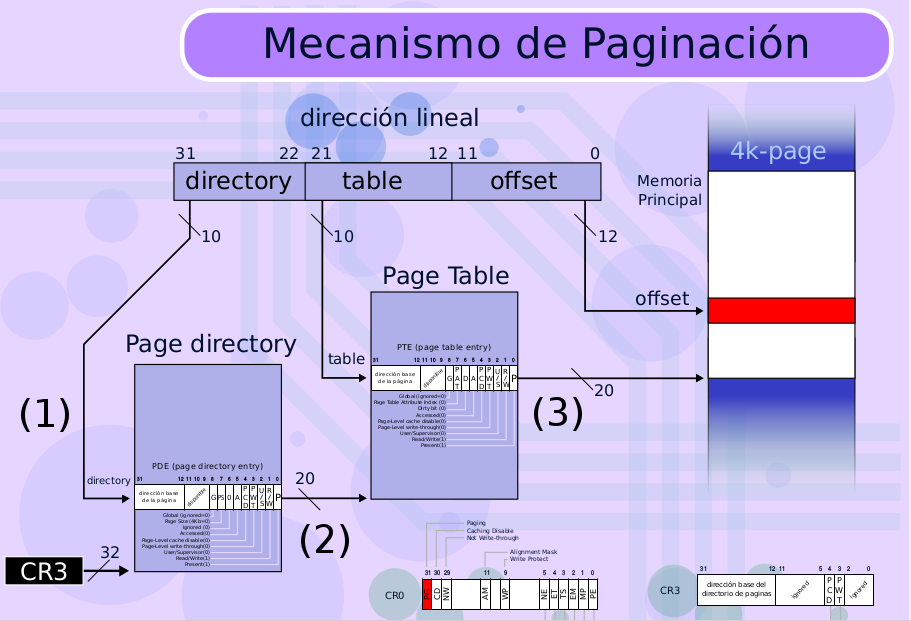
\includegraphics[width=100mm]{imagenes/paginacion.png}
\caption{Mapeo de P\'aginas}
\end{figure}

\par Para mapear p\'aginas \texttt{mmu_map_page} toma una direcci\'on virtual, una f\'isica, un selector del directorio a mapear, y dos par\'ametros de permisos (user/supervisor, read/write).

\par El algoritmo de mapeo es el siguiente:

\begin{itemize}
\item Primero limpiamos los bits de permisos del selector y obtenemos el directorio.
\item  Luego buscamos la tabla de p\'aginas para mapear. Para esto avanzamos hasta su descriptor sumando a la direcci\'on base el offset indicado en los primeros 10 bits de la direcci\'on virtual.
\item Si dicho descriptor tiene el bit presente en 1, shifteamos su base y obtenemos la direcci\'on del comienzo de la tabla que buscamos; sino, creamos la tabla y asignamos su base al descriptor del directorio.
\item Finalmente avanzamos hasta el descriptor de la p\'agina, seteamos el bit de presente junto con los dem\'as permisos y su base ser\'a la direcci\'on f\'isica shifteada 12 a la derecha.
\end{itemize}

\begin{lstlisting} [caption={Mapeo de p\'aginas}],label=mmuMapPage] 
void mmu_map_page(unsigned int virtual, unsigned int cr3, unsigned int fisica, char sup, char rw){
	page_directory_entry* page_dir = (page_directory_entry*) ((cr3 >> 3) << 3);

	page_table_entry* pte;
	if (page_dir[PDE_INDEX(virtual)].p){
		pte = (page_table_entry*) (page_dir[PDE_INDEX(virtual)].base << 12);
	} else {
		pte = (page_table_entry*) mmu_proxima_pagina_fisica_libre();
		page_dir[PDE_INDEX(virtual)].base = ((unsigned int) pte) >> 12;
		page_dir[PDE_INDEX(virtual)].p = 1;
		page_dir[PDE_INDEX(virtual)].rw = 1;
		page_dir[PDE_INDEX(virtual)].s = 1;
	}
	pte[PTE_INDEX(virtual)].p = 1;
	pte[PTE_INDEX(virtual)].rw = rw;
	pte[PTE_INDEX(virtual)].s = sup;
	pte[PTE_INDEX(virtual)].pwt = 0;
	pte[PTE_INDEX(virtual)].pcd = 0;
	pte[PTE_INDEX(virtual)].a = 0;
	pte[PTE_INDEX(virtual)].d = 0;
	pte[PTE_INDEX(virtual)].pat = 0;
	pte[PTE_INDEX(virtual)].g = 0;
	pte[PTE_INDEX(virtual)].disp = 0;
	pte[PTE_INDEX(virtual)].base = fisica >> 12;		
	tlbflush();
}
\end{lstlisting}

\par \texttt{mmu_unmap_page} toma la direcci\'on virtual y el cr3 del directorio. Para desmapear accedemos al descriptor de dicha p\'agina y seteamos el bit de presente en 0.

\begin{lstlisting} [caption={Desmapeo de p\'aginas}],label=mmuUnmap] 
void mmu_unmap_page(unsigned int virtual, unsigned int cr3){
	page_directory_entry* page_dir = (page_directory_entry*) ((cr3 >> 3) << 3);
	page_table_entry* pte = (page_table_entry*) (page_dir[PDE_INDEX(virtual)].base << 12);
	pte[PTE_INDEX(virtual)].p = 0;
}
\end{lstlisting}

\newpage
\subsubsection*{Inicialización de directorios y tablas para Zombis}

\par \texttt{mmu_inicializar_dir_zombi} toma el tipo de zombie que el jugador quiere inicializar y la posici\'on (x,y) donde se quiere inicializarlo y devuelve la direcci\'on del directorio creado para este zombi.

\par La inicializaci\'on del directorio y tabla de p\'aginas para dicho zombi respetan el formato presentado en el enunciado:

\begin{figure}[ht!]
\centering
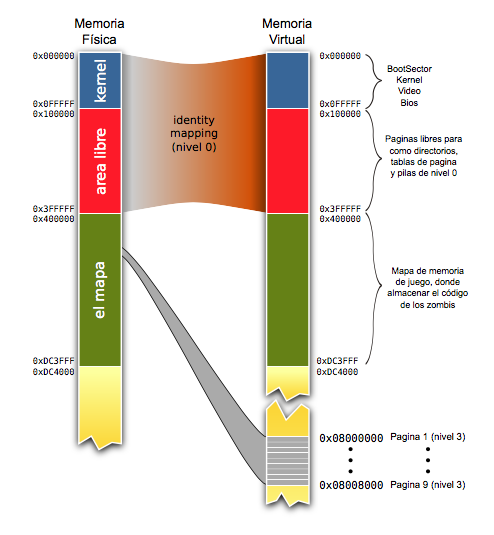
\includegraphics[width=100mm]{imagenes/memoriatarea.png}
\caption{Mapa de memoria de la Tarea.}
\end{figure}

\par La descripci\'on del algoritmo es la siguiente:

\begin{itemize}
\item Para obtener el nuevo directorio, pedimos una p\'agina libre y mapeamos con identity mapping todas las p\'aginas entre 0x000000 y 0x03FFFFF.
\item Luego, obtenemos la direcci\'on f\'isica a la que corresponde esa posici\'on (entre 0x400000 y 0xDC3FFF) y copiamos el c\'odigo del zombi (que dependiendo del tipo, est\'a en alguna direcci\'on f\'isica fija). Cabe aclarar que primero mapeamos en el directorio del kernel la p\'agina destino (que no est\'a mapeada), y luego de copiar el c\'odigo la desmapeamos.
\item Por \'ultimo, mapeamos las 9 p\'aginas virtuales del zombi a sus correspondientes f\'isicas.
\end{itemize}

\newpage
\begin{lstlisting} [caption={Inicializaci\'on directorio y tabla de p\'aginas del zombi}],label=mmuDirZombi] 
unsigned int mmu_inicializar_dir_zombi(unsigned short x, unsigned short y, zombie z) {
	page_directory_entry* dir_pagina = (page_directory_entry*) mmu_proxima_pagina_fisica_libre();
	inicializar_con_identity_mapping(dir_pagina);

	unsigned int* origin;
	switch (z) {
		case A_MONK:
			origin = (unsigned int*)0x10000;
			break;
        case A_SUICIDE_UNIT:
        	origin = (unsigned int*)0x11000;
        	break;
        case A_DRUNK_DRIVER:
        	origin = (unsigned int*)0x12000;
        	break;
        case B_MONK:
        	origin = (unsigned int*)0x13000;
        	break;
        case B_SUICIDE_UNIT:
        	origin = (unsigned int*)0x14000;
        	break;
        case B_DRUNK_DRIVER:
        	origin = (unsigned int*)0x15000;
        	break;
    }

	unsigned int* dest = (unsigned int*) mmu_get_map_position(x, y); 
	mmu_map_page((unsigned int)dest, rcr3(), (unsigned int)dest, 0, 1);
	unsigned int i;
	for (i=0; i<1024; i++){
		dest[i] = origin[i];
	}
	
	mmu_unmap_page((unsigned int)dest, rcr3());

	if (x == POS_INIT_ZOMBI_A){
		mmu_map_adjacent_to_zombi(0, (unsigned int) dir_pagina, x, y);
	} else if (x == POS_INIT_ZOMBI_B){
		mmu_map_adjacent_to_zombi(1, (unsigned int) dir_pagina, x, y);
	}

	return (unsigned int)dir_pagina;
}
\end{lstlisting}

\par Para manejar el video convenientemente, nos pareci\'o \'util hacer una funci\'on para obtener la p\'agina del video asociada a una coordenada.

\begin{lstlisting} [caption={Obtener p\'agina de coordenada}],label=mmuObtenerPaginaDedir] 
unsigned int mmu_get_map_position ( int x,  int y) {
	return 0x400000 + (MOD(y,44) * 78 + x) * PAGE_SIZE;
}
\end{lstlisting}

\newpage
\par Finalmente, \texttt{mmu_map_adjacent_to_zombi} mapea las 9 p\'aginas virtuales del zombie a las 9 p\'aginas f\'isicas del video.

\begin{lstlisting} [caption={Mapeo de zombi a una coordenada en el mapa}],label=mmuMapDirZombi] 
void mmu_map_adjacent_to_zombi(unsigned int player, unsigned int dir_pagina, unsigned int x, unsigned int y){
	mmu_map_page(VIRTUAL_COD_ZOMBIE_1, dir_pagina, mmu_get_map_position(x, y), 1, 1);
	if (player == 0) {
		mmu_map_page(VIRTUAL_COD_ZOMBIE_2, dir_pagina, mmu_get_map_position(x+1, y), 1, 1);
		mmu_map_page(VIRTUAL_COD_ZOMBIE_3, dir_pagina, mmu_get_map_position(x+1, y+1), 1, 1);
		mmu_map_page(VIRTUAL_COD_ZOMBIE_4, dir_pagina, mmu_get_map_position(x+1, y-1), 1, 1);
		mmu_map_page(VIRTUAL_COD_ZOMBIE_5, dir_pagina, mmu_get_map_position(x, y+1), 1, 1);
		mmu_map_page(VIRTUAL_COD_ZOMBIE_6, dir_pagina, mmu_get_map_position(x, y-1), 1, 1);
		mmu_map_page(VIRTUAL_COD_ZOMBIE_7, dir_pagina, mmu_get_map_position(x-1, y), 1, 1);
		mmu_map_page(VIRTUAL_COD_ZOMBIE_8, dir_pagina, mmu_get_map_position(x-1, y-1), 1, 1);
		mmu_map_page(VIRTUAL_COD_ZOMBIE_9, dir_pagina, mmu_get_map_position(x-1, y+1), 1, 1);
	} else {
		mmu_map_page(VIRTUAL_COD_ZOMBIE_2, dir_pagina, mmu_get_map_position(x-1, y), 1, 1);
		mmu_map_page(VIRTUAL_COD_ZOMBIE_3, dir_pagina, mmu_get_map_position(x-1, y-1), 1, 1);
		mmu_map_page(VIRTUAL_COD_ZOMBIE_4, dir_pagina, mmu_get_map_position(x-1, y+1), 1, 1);
		mmu_map_page(VIRTUAL_COD_ZOMBIE_5, dir_pagina, mmu_get_map_position(x, y-1), 1, 1);
		mmu_map_page(VIRTUAL_COD_ZOMBIE_6, dir_pagina, mmu_get_map_position(x, y+1), 1, 1);
		mmu_map_page(VIRTUAL_COD_ZOMBIE_7, dir_pagina, mmu_get_map_position(x+1, y), 1, 1);
		mmu_map_page(VIRTUAL_COD_ZOMBIE_8, dir_pagina, mmu_get_map_position(x+1, y+1), 1, 1);
		mmu_map_page(VIRTUAL_COD_ZOMBIE_9, dir_pagina, mmu_get_map_position(x+1, y-1), 1, 1);
	}
}
\end{lstlisting}

\newpage
\section{Ejercicio 5}
	\subsubsection*{Asociamos las rutinas de interrupcion a la de reloj, teclado y syscall}
\par{Para inicializar las interrupciones de teclado y reloj utilizamos la misma macro nombrada en el Ejercicio2, llamada IDT\_ENTRY\_SYSTEM. Para inicializar la entrada de la syscall creamos una macro parecida a la IDT\_ENTRY\_SYSTEM pero con distintos atributos. A esta la llamaremos IDT\_ENTRY\_USER y la describimos de la siguiente manera:}

\begin{lstlisting} [caption={Macro IDT\_ENTRY\_USER}],label=idtDesc] 
#define IDT_ENTRY_USER(numero)                                         
    idt[numero].offset_0_15 = (unsigned short) ((unsigned int)(&_isr ## numero) & (unsigned int) 0xFFFF); 
    idt[numero].segsel = (unsigned short) 0x0040;
    idt[numero].attr = (unsigned short) 0xEE00;
    idt[numero].offset_16_31 = (unsigned short) ((unsigned int)(&_isr ## numero) >> 16 & (unsigned int) 0xFFFF);
\end{lstlisting}


\\
\subsubsection*{Rutina atenci\'on de clock}
\par{Creamos la rutina de atenci\'on de clock, en esta llamamos a pr\'oximo reloj que se encarg\'a de avanzar el dibujo del clock y luego avisamos al PIC que la interrupci\'on fue atendida mediante call fin\_intr\_pic1. Luego ser\'a modificada para el uso del scheduler.}
\begin{lstlisting} [caption={Rutina atenci\'on clock}],label=idtDesc] 
_isr32:
    pushad
    call proximo_reloj
    call fin_intr_pic1
    popad
    iret

\end{lstlisting}

\subsubsection*{Rutina de atenci\'on de teclado}
\par{Creamos la rutina de atenci\'on de teclado. Esta rutina toma el valor de la tecla presionada y compara este valor con los de las teclas correspondientes al juego. Luego hace un jump a el c\'odigo de esa tecla en particular. A continuaci\'on un ejemplo de la tecla $a$:}

\begin{lstlisting} [caption={Rutina atenci\'on teclado}],label=idtDesc] 
_isr33:
    pushad
    xor eax, eax
    in al, 0x60
    
    cmp al, 0x1e
    je .a

.a: ; A hacia izq
    mov ebx, -1
    push ebx
    mov ebx, 0
    push ebx
    call game_change_zombie
    add esp, 8
    jmp .fin


    .fin:
        call fin_intr_pic1
        popad
        iret
\end{lstlisting}

\\
\par{El c\'odigo real es m\'as largo, contiene comparaciones y etiquetas para todas las teclas que son parte del juego.}

\subsubsection*{Rutina atenci\'on syscall}
\par{La siguiente es la rutina de atenci\'on de la interrupci\'on 0x66, este es el c\'odigo ya modificado para atender la syscall. Luego de mover al zombie hacemos un salto a la tarea idle.}
\begin{lstlisting} [caption={Rutina atenci\'on de  syscall}],label=idtDesc] 
_isr102:
    pushad
    push eax
    call game_move_current_zombi
    pop eax
    ;jump a la tarea idle
    jmp 0x70:0xFAFAFA    
    popad
    iret

\end{lstlisting}


\newpage
\section{Ejercicio 6}
	\subsection*{Inicializaci\'on de descriptores de TSS en la GDT}
\par{Para inicializar los Task State Segment (TSS) debemos agregar sus descriptores a la GDT. La mayor\'ia de las variables del descriptor de TSS (gdt_entry) son iguales para todas las TSS:}

\begin{lstlisting} [caption={Descriptor de TSS (gdt_entry)},label=idtEntry]
gdt[GDT_IDX_TAREA] = (gdt_entry) {
        (unsigned short)    0x0068,         /* limit[0:15]  */
        (unsigned short)    0x0000,         /* base[0:15]   */
        (unsigned char)     0x00,           /* base[16:23]  */
        (unsigned char)     0x09,           /* type         */
        (unsigned char)     0x00,           /* s            */
        (unsigned char)     0x00,           /* dpl          */
        (unsigned char)     0x00,           /* p            */
        (unsigned char)     0x00,           /* limit[16:19] */
        (unsigned char)     0x00,           /* avl          */
        (unsigned char)     0x00,           /* l            */
        (unsigned char)     0x00,           /* db           */
        (unsigned char)     0x00,           /* g            */
        (unsigned char)     0x00,           /* base[24:31]  */
    }
\end{lstlisting}

\par{A diferencia de las tareas-zombie, la Idle y la inicial comienzan con el bit de presente en 1. Por otro lado, la base de la tss se setea en el momento de inicializar cada tarea, cuando conocemos su posicion en memoria.}
\subsection*{Inicializaci\'on de TSSs}
\par{Para representar a las tss, contamos con el siguiente struct:}

\begin{lstlisting} [caption={Descriptor de TSS (gdt_entry)},label=idtEntry]
typedef struct str_tss {
    unsigned short  ptl;            unsigned short  unused0;
    unsigned int    esp0;
    unsigned short  ss0;            unsigned short  unused1;
    unsigned int    esp1;
    unsigned short  ss1;            unsigned short  unused2;
    unsigned int    esp2;
    unsigned short  ss2;            unsigned short  unused3;
    unsigned int    cr3;
    unsigned int    eip;
    unsigned int    eflags;
    unsigned int    eax;
    unsigned int    ecx;
    unsigned int    edx;
    unsigned int    ebx;
    unsigned int    esp;
    unsigned int    ebp;
    unsigned int    esi;
    unsigned int    edi;
    unsigned short  es;             unsigned short  unused4;
    unsigned short  cs;             unsigned short  unused5;
    unsigned short  ss;             unsigned short  unused6;
    unsigned short  ds;             unsigned short  unused7;
    unsigned short  fs;             unsigned short  unused8;
    unsigned short  gs;             unsigned short  unused9;
    unsigned short  ldt;            unsigned short  unused10;
    unsigned short  dtrap;          unsigned short  iomap;
} __attribute__((__packed__, aligned (8))) tss;
\end{lstlisting}

\par{En el caso de la tss de la tarea inicial no es necesario setear ninguna variable, solo se usa para guardar el contexto al saltar a la Idle y nunca se vuelve. Para la tss de la Idle las variables se setean de acuerdo a la consigna del tp.}
\par{Por otro lado, contamos con la funci\'on tss_inicializar_zombie que se encarga inicializar una tarea lanzada por un jugador. Primeramente, busca un slot libre en el arreglo gdt_indexes_tasks en la estructura info_jugador (explicada de el ejercicio 7). Con \'indice del slot libre accedemos a su descriptor de segmento en la gdt para setear el bit de presente en 1 y su base a que apunte a donde esta la tss. Posteriormente inicializamos el directorio de p\'agina de la tarea y pedimos una p\'agina libre para usarla como stack de nivel 0. Por \'ultimo seteamos las variables de la tss:}

\begin{lstlisting} [caption={Descriptor de TSS (gdt_entry)},label=idtEntry]
unsigned int dir_z = mmu_inicializar_dir_zombi(x, y, z);
unsigned int ss = mmu_proxima_pagina_fisica_libre();
tss_zombi->esp0 = ss + PAGE_SIZE;
tss_zombi->ss0 = GDT_IDX_DAT_KERNEL<<3;
tss_zombi->cr3 = dir_z;
tss_zombi->eip = VIRTUAL_COD_ZOMBIE_1;
tss_zombi->eflags = 0x202;
tss_zombi->cs = GDT_IDX_COD_USER << 3 | 0x3;
tss_zombi->es = GDT_IDX_DAT_USER << 3 | 0x3;
tss_zombi->ss = GDT_IDX_DAT_USER << 3 | 0x3;
tss_zombi->ds = GDT_IDX_DAT_USER << 3 | 0x3;
tss_zombi->fs = GDT_IDX_DAT_USER << 3 | 0x3;
tss_zombi->gs = GDT_IDX_DAT_USER << 3 | 0x3;
tss_zombi->esp = VIRTUAL_COD_ZOMBIE_1 + PAGE_SIZE;
tss_zombi->ebp = VIRTUAL_COD_ZOMBIE_1 + PAGE_SIZE;
\end{lstlisting}

\subsection*{Carga de  tarea inicial y salto a la Idle}
\par{Para cargar la tarea inicial tenemos que setear el task register:}
\begin{lstlisting} []
mov ax, 0x0D<<3
ltr ax
\end{lstlisting}
\par{Posteriormente, para pasar a la tarea Idle simplemente hacemos:}
\begin{lstlisting} []
jmp 0x70:0xFAFAFA
\end{lstlisting}
\par{Donde 0x70 es el selector de segmento de la tarea.}
    
\newpage
\section{Ejercicio 7}
	\subsubsection*{Estructuras del Scheduler}
\par Las variables de nuestro scheduler son las siguientes:

\begin{lstlisting} [caption={Variables del Scheduler},label=SchedulerVars]
info_player playerA;
info_player playerB;
int playerActual;
int isIdle;
\end{lstlisting}

\par $playerActual$ indica cu\'al es el jugador que tiene el turno actualmente; $info\_playerA$ e $info\_playerB$ guardan la informaci\'on relevante al jugador. Finalmente, nos pareci\'o relevante agregar la variable $isIdle$, que indica si la tarea actual es la Idle.

\begin{lstlisting} [caption={Informaci\'on del zombi},label=infoZombi]
typedef struct str_info_zombie {
    zombie  type;
    unsigned short  x;
    unsigned short  y;
    unsigned short reloj_actual;
} __attribute__((__packed__, aligned (16))) info_zombie;
\end{lstlisting}

\par \texttt{info_zombie} guarda su posici\'on actual la pantalla, su tipo (que es un enum), y su reloj actual (que es un n\'umero entre 0 y 3 que indica qu\'e caracter del reloj tiene dibujado el zombi en este momento). 

\begin{lstlisting} [caption={Informaci\'on del jugador},label=infoPlayer]
typedef struct str_info_player {
    zombie  selected_type;
    unsigned short  y;
    unsigned short cant_lanzados;
    unsigned short gdt_indexes_tasks[CANT_ZOMBIS];
    info_zombie info_zombies[CANT_ZOMBIS];
    unsigned short curr_zombie;
    unsigned short puntos;
} __attribute__((__packed__, aligned (16))) info_player;
\end{lstlisting}

\par Por otro lado, \texttt{info_player} guarda el tipo de zombie seleccionado actualmente, la posici\'on del jugador en el eje vertical, la cantidad de zombies lanzados, y sus puntos. Lo m\'as interesante es \texttt{gdt_indexes_tasks} que es un arreglo de selectores de la gdt, donde el i-\'esimo selector se corresponde con el i-\'esimo zombie de info\_zombies. Por \'ultimo, curr\_zombie indica el \'indice del zombie actual del jugador.

\newpage

\subsubsection*{Task switch}

\par{Como vemos en la figura 3, las tareas de los zombies deben ir alternandose entre el jugador A y el B. Adem\'as los zombies de cada jugador deben correr uno tras otro y de manera c\'iclica.}

\begin{figure}[ht!]
\centering
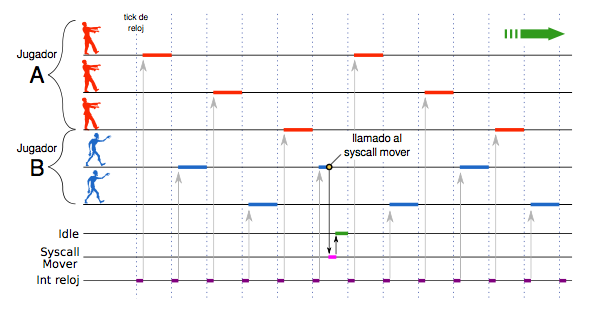
\includegraphics[width=100mm]{imagenes/scheduler.png}
\caption{Ejemplo de funcionamiento del Scheduler}
\end{figure}

\par{Lo que hacemos entonces es preguntar en cada interrupci\'on de reloj qui\'en es el pr\'oximo \'indice de tarea a ejecutar y hacemos el jump a ella. En caso que el scheduler nos devuelva el \'indice 0 no haremos nada, nos quedamos en la tarea actual. A continuaci\'on el c\'odigo de la interrupci\'on de clock.}

\begin{lstlisting} [caption={Interrupci\'on de clock},label=infoPlayer]
_isr32:
    pushad

    call proximo_reloj
    mov eax, [inDebugMode] 
    mov esi, [debugScreenOpen]
    and eax, esi
    cmp eax, 1
    je .nojump  ;si esta en modo debug con la pantalla de debug abierta no hago nada


    call sched_proximo_indice

    cmp ax, 0
    je .nojump
        push eax
        call girar_reloj_actual
        pop eax
        mov [selector], ax
        call fin_intr_pic1
        jmp far [offset]
        jmp .end

    .nojump:
    call fin_intr_pic1

    .end:
    popad
    iret
\end{lstlisting}

\\
\par{Nos salteamos las lineas que hablan del debugger ya que este ser\'a explicado m\'as adelante. Como vemos hacemos un $call$ a $sched\_proximo\_indice$ como habiamos dicho y a continuaci\'on saltamos a esa tarea. En caso de ser 0 no hacemos ning\'un $jmp$.}
\par{Lo que hace $sched\_proximo\_indice$ es tomar la informaci\'on de playerActual para saber quien es el siguiente jugador. Si el jugador opuesto al actual no tiene tareas en su lista de $gdt\_index\_tasks$ (osea tiene todos 0), entonces no se cambiar\'a el $playerActual$. En caso contrario, el player actual pasar\'a a el otro jugador.}
\par{Si este es el primer zombie que se lanza (caso en que zombie inicial del player ser\'a 32) entonces verifico que haya zombies en la lista de indices, puesto que si no los hay es por que a\'un no se han lanzado zombies y por ende no hay que saltar a ninguna tarea de este jugador. Si hay zombies en la lista entonces el primer zombie ser\'a el proximo a saltar.}
\par{Si no estamos en el caso anterior entonces lo que hay que hacer es recorrer la lista de \'indices busucando el primero que sea distinto de 0. Si se llega al final del arreglo se empieza desde el inicio. Si se encuentra de esta manera una tarea distinta a la actual para este jugador entonces ser\'a ese \'indice el que se devuelva y esa tarea a la que se salte.}
\par{Si se dio toda la vuelta y se lleg\'o al mismo zombie que el actual entonces tenemos que preguntarnos si estamos en la tarea Idle ya que si estamos en la tarea idle entonces vuelve a ser el turno de este zombie, pero si no estamos en la tarea idle entonces no debemos hacer nada y devolver 0 ya que actualmente estamos en el turno de ese zombie.}



\newpage
\subsubsection*{Syscall mover}

\par La syscall mover es la \'unica prove\'ida por el sistema, y est\'a mapeada a la interrupci\'on 0x66.
\par La codificaci\'on de desplazamientos es la siguiente:

\begin{figure}[ht!]
\centering
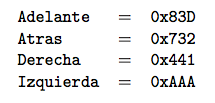
\includegraphics[width=40mm]{imagenes/movercodes.png}
\caption{C\'odigos de mover}
\end{figure}

\par Atendemos la interrupci\'on en assembler y llamamos a \texttt{game_move_current_zombi} en C, cuyo \'unico par\'ametro es la direcci\'on en la que quiere moverse el zombie, y su funcionamiento es:

\begin{itemize}
\item 1. Dada la direcci\'on pasada por par\'ametro, obtenemos la p\'agina virtual a donde se va a mover.
\end{itemize}

\begin{lstlisting} [caption={Syscall mover - obtener origen y destino},label=moverOrigen]
    unsigned int* orig = (unsigned int*) VIRTUAL_COD_ZOMBIE_1;
    unsigned int* dest;
	switch (dir) {
	case IZQ:
    	dest = (unsigned int*)VIRTUAL_COD_ZOMBIE_6;
		break;
    case DER:
    	dest = (unsigned int*)VIRTUAL_COD_ZOMBIE_5; 
    	break;
    case ADE:
    	dest = (unsigned int*)VIRTUAL_COD_ZOMBIE_2;
    	break;
    case ATR:
    	dest = (unsigned int*)VIRTUAL_COD_ZOMBIE_7;    
    	break;
    }
\end{lstlisting}

\begin{itemize}
\item 2. Copiamos la p\'agina entera del c\'odigo del zombie, a su p\'agina f\'isica de destino. Esto es copiando su p\'agina virtual actual a su p\'agina virtual destino, porque ambas est\'an mapeadas sus correspondientes f\'isicas.
\end{itemize}

\begin{lstlisting} [caption={Syscall mover - copiar c\'odigo del zombie},label=moverCopiar]
    int i;
    for(i=0; i<1024; i++){
    	dest[i] = orig[i];
    }
\end{lstlisting}

\begin{itemize}
\item 3. Calculamos la nueva posici\'on (x, y) (tomando en cuenta qu\'e jugador es el actual, y la circularidad del mapa).
\end{itemize}

\begin{lstlisting} [caption={Syscall mover - calcular nueva (x, y)},label=moverNuevaXY]
info_player* current_player = get_current_player();
    unsigned short current_zombie = current_player->curr_zombie;
    unsigned short x_orig = (current_player->info_zombies[current_zombie]).x;
    unsigned short y_orig = (current_player->info_zombies[current_zombie]).y;
    unsigned short x_dst = x_orig;
    unsigned short y_dst = y_orig;

    if(y_dst==0 || y_dst==43){
        if ((dir == IZQ && playerActual == 0) || (dir == DER && playerActual == 1)) {
            y_dst=43;
        } else if ((dir == DER && playerActual == 0) || (dir == IZQ && playerActual == 1)) {
            y_dst=0;
        } else if ((dir == ADE && playerActual == 0) || (dir == ATR && playerActual == 1)) {
            x_dst++;

        } else if ((dir == ATR && playerActual == 0) || (dir == ADE && playerActual == 1)) {
            x_dst--;
        }
    }else{
        if ((dir == IZQ && playerActual == 0) || (dir == DER && playerActual == 1)) {
            y_dst--;
        } else if ((dir == DER && playerActual == 0) || (dir == IZQ && playerActual == 1)) {
            y_dst++;
        } else if ((dir == ADE && playerActual == 0) || (dir == ATR && playerActual == 1)) {
            x_dst++;

        } else if ((dir == ATR && playerActual == 0) || (dir == ADE && playerActual == 1)) {
            x_dst--;
        }
    }   

\end{lstlisting}

\begin{itemize}
\item 4. Asignamos al zombie a su nueva posici\'on.
\end{itemize}

\begin{lstlisting} [caption={Syscall mover - asignar nuevas coordenadas al zombie},label=moverAsignarCoordenadas]
    (current_player->info_zombies[current_zombie]).x = x_dst;
    (current_player->info_zombies[current_zombie]).y = y_dst;
\end{lstlisting}

\begin{itemize}
\item 5. De llegar a un borde, sumamos punto, matamos al zombie, y terminamos la ejecuci\'on del algoritmo.
\end{itemize}

\begin{lstlisting} [caption={Syscall mover - sumar punto y matar zombie},label=moverSumarYMatar]
    if(x_dst==1){
        game_sumar_punto(1/*jugador azul*/);
        game_matar_zombie_actual();
        return;
    }
    if(x_dst==78){
        game_sumar_punto(0/*jugador rojo*/);
        game_matar_zombie_actual();
        return;
    }
\end{lstlisting}

\begin{itemize}
\item 6. Remapeamos todas las p\'aginas virtuales del zombie teniendo en cuenta su nueva posici\'on (x, y).
\end{itemize}

\begin{lstlisting} [caption={Syscall mover - remapear las p\'aginas del zombie (vease Ej. 4)},label=moverRemapear]
    /* remapear sus direcciones */
    mmu_map_adjacent_to_zombi(playerActual, rcr3(), x_dst, y_dst);
\end{lstlisting}

\begin{itemize}
\item 7. Por \'ultimo imprimimos el cambio en pantalla y seteamos la tarea idle en el scheduler.
\end{itemize}

\begin{lstlisting} [caption={Syscall mover - Imprimir en pantalla y setear Idle},label=moverImprimir]
    print_move_zombie(playerActual, x_orig, y_orig, x_dst, y_dst, (current_player->info_zombies[current_zombie]).type);
    isIdle=1;
\end{lstlisting}

\subsubsection*{Modo debug}
\par{Para implementar el modo debug en nuestro juego nos encontramos con tres problem\'aticas:}
\begin{enumerate}
\item C\'omo recuperar los valores de algunos registros que son modificados cuando se produce la interrupci\'on
\item Guardar el estado de la pantalla del juego antes de que aparezca el cartel, para luego poder restaurarla
\item Que otras tareas no se sigan ejecutando y que los jugadores no puedan realizar acciones cuando esta la pantalla de debug abierta
\end{enumerate}

\par{Para guardar el estado de los registros al momento de producirse una interrupci\'on contamos con el struct debug_info. La mayor\'ia de los registros siguen iguales despu\'es de producida la interrupci\'on. Algunos son modificados, pero antes son apilados en el stack. El estado del stack despues de transferir el control al handler de interrupciones es el siguiente:}

\begin{figure}[ht!]
\centering
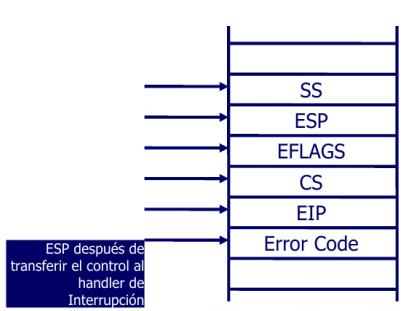
\includegraphics[width=70mm]{imagenes/stack.png}
\caption{Stack al momento de entrar al handler de interrupciones}
\end{figure}

\par{Por otro lado, para poder guardar el estado de la pantalla antes de que aparezca el cartel del debugger contamos con la variable $backup$ (matriz de $ca$ que se corresponde con la pantalla), la funci\'on $backup\_screen$ (que guarda la pantalla en la variable) y la funci\'on $backup\_restore\_screen$ (que escribe en la pantalla lo que hay guardado en la variable).}

\par{Por \'ultimo, para poder manejar las tareas en modo debug contamos con dos variables globales: inDebugMode, que indican si se est\'a en modo debug, y $debugScreenOpen$, que indica si la ventana de debug est\'a abierta. Al producirse la excepci\'on se setea $debugSreenOpen$ en 1, se muestra la pantalla de debug y se salta a la tarea Idle. Dentro de la interrupci\'on de clock, si $inDebugMode$ y $debugScreenOpen$ est\'an seteados, no se salta a la pr\'oxima tarea. Dentro de la interrupci\'on de teclado, si $inDebugMode$ y $debugScreenOpen$ est\'an seteados, solamente la tecla 'y' produce un cambio en el juego (cerrar la pantalla de debug).}

\newpage
\section{Conclusiones}
	\par Para concluir el informe, nos parece que este trabajo nos ayud\'o a entender muchos mecanismos claves de un sistema operativo, como por ejemplo el manejo de memoria, manejo de tareas y atenci\'on de interrupciones.
\par Y, de m\'as est\'a decir que sabemos que un sistema operativo real comprende una complejidad bastante superior al nuestro, pero confiamos que este trabajo nos sent\'o una buena base para ayudarnos a entender un sistema real.

\end{document}

